%conceitos básicos deviam ser mais abstratos, e não falar a respeito de características da placa/processador físico.

\chapter{EPOS}
%memory chunks, address spaces
%free memory list
%make a diagram showing how MMU alloc a physical page, and how the heap lends pages that were already allocted in the MMU's point of view.
%least amount of interrupts possible
%alarm's diagram
%alarm's queue

%epos mote

%cite some works done using EPOS (specially giovani's).


%source: http://epos.lisha.ufsc.br/EPOS+User+Guide
\section{EPOS}

EPOS (Embedded Parallel Operating System) é um sistema operacional orientado a aplicação, cujo design chama-se ADESD (\emph{Application-Driven Embedded System Design Method}), proposto por Fröhlich \cite{guto_thesis}. A ideia central do EPOS é prover um sistema operacional mínimo, de modo a minimizar o \emph{overhead} da existência de um sistema operacional, deixando o processador livre para executar a aplicação do desenvolvedor \cite{epos_user_guide}.

Como o objetivo é criar um ambiente em que o desenvolvedor possa rapidamente produzir suas aplicações, EPOS provê vários utilitários comumente usados em aplicações, como filas, listas, tabelas de hashs, vetores, semáforos, OStream (para imprimir na tela), números aleatórios, cálculo de CRC e etc. Além destes utilitários, EPOS também provê uma série de componentes como threads, alarmes, cronometros, \emph{heaps} e meios para acessar a rede (internet).

\section{Arquitetura do EPOS}

\textbf{Mediadores de Hardware:} Dentro da arquitetura do EPOS há o conceito de mediadores de hardware, que são os componentes (ou classes) dependentes de plataforma. Idealmente, as únicas classes que precisam ser modificadas e/ou reimplementadas são os mediadores. Há mediadores específicos da placa, como por exemplo Pandaboard, Zedboard e etc; abstraídos sob o nome de \emph{machine} e mediadores específicos de um processador, abstraídos sob o nome de \emph{architecture}. No código do EPOS, estes mediadores encontram-se nas pastas \emph{mach} e \emph{arch}.
% Fonte: Hardware Mediators: A Portability Artifact for Component-based Systems
% HAL vs Virtualização vs Mediadores

Mediadores de hardware são uma alternativa ao tradicional uso de VMs\footnote{Virtual Machines.} e de HAL\footnote{Hardware Abstraction Layer}, proposta por Fröhlich em seu trabalho \emph{Application-Oriented System Design} \cite{guto_thesis}. O problema do uso de VMs é o seu \emph{overhead} causado devido à tradução das operações da VM em código nativo. Já o uso de um HAL incorre no problema da manutenibilidade e dificuldade de adapção à novas arquiteturas muito distintas entre si \cite{hw_mediators}. O HAL não conseguiu passar pela ``prova do tempo'', e já está sendo considerado obsoleto por distribuições GNU/Linux populares, como o 
Ubuntu\footnote{\url{http://www.linux-magazine.com/Online/News/Ubuntu-10.04-Alpha-2-Removes-HAL}}, sendo chamado de ``uma grande não-manutenível bagunça monolítica''\footnote{\url{https://wiki.ubuntu.com/Halsectomy}}.



\textbf{Traits:} Traits são classes onde é possível configurar certos componentes do EPOS em tempo de compilação. Lá é possível, por exemplo, definir o tamanho da \emph{stack} e \emph{heap} do sistema, a sua frequência de \emph{clock} bem como ativar ou desativar certas funções do sistema. Esta classe normalmente precisa ser alterada em um porte, mesmo ela não sendo um mediador de hardware, pois eles usam as configurações descritas nos traits.

\textbf{Interface Infladas: } Um conceito importante da arquitetura do EPOS é a Interface Inflada. %http://www.inf.ufsc.br/~guto/publications/aoos.pdf
Em sistemas orientados a aplicação, famílias de abstrações são frequentemente tratadas como entidades únicas, algo que pode ser vantajoso para o programador da aplicação, já que este não precisaria se preocupar com qual membro em específico desta família ele precisaria usar \cite{guto_thesis}.

Interface inflada basicamente é uma interface que declara os métodos de todas as classes que derivam dela, exportanto assim todos os métodos daquela família de abstrações, como mostra a figura \ref{fig:inflated}. Deste modo, o desenvolvedor de aplicativo poderia escrever a aplicação inteira em termos da interface inflada, relegando a tarefa de configuração do sistema a um utilitário automatizado. Tal utilitário poderia, através de uma análise sintática do código fonte, escolher quais os membros mais apropriados da família exportada serão associados no momento da compilação \cite[p.~56]{guto_thesis}.

%write about specifics from timers
\begin{figure}[ht!]
	\label{fig:inflated}
    \centering
    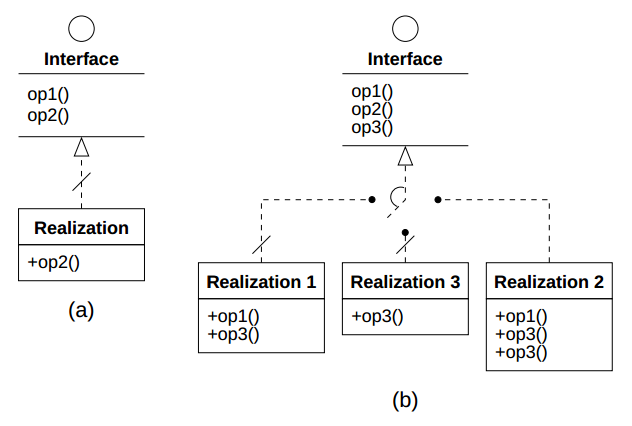
\includegraphics[width=7.5cm]{figuras/inflated_interface}
    \caption{Exemplos de uso de interfaces infladas \cite{guto_thesis}.}
\end{figure}

